% -----------------------------*- LaTeX -*------------------------------
\documentclass[UTF8]{report}
% ------------------------------------------------------------------------
% Packages
% ------------------------------------------------------------------------
\usepackage{ctex} % 支持中文
\usepackage[body={7in, 9in},left=1in,right=1in]{geometry} % 改变页边距
\usepackage{amsmath} % AMS 的数学宏包
\usepackage{amsfonts} % AMS 的数学字体宏包
\usepackage{amssymb} % AMS 符号库
\usepackage{bm} % 数学公式中的黑斜体h
\usepackage{amsthm} % AMS 的定理环境宏包
\usepackage{graphicx} % 插图
\usepackage{subfigure} % 插子图
\usepackage{nicefrac} % 好看的分数
\usepackage{mathrsfs} % mathscr font
\usepackage{caption} % caption
\usepackage{algorithm,algorithmicx} % 伪代码支持宏包
\usepackage[noend]{algpseudocode} % 伪代码
\usepackage{fancyhdr} % 设置页眉、页脚
\usepackage{adjustbox} % 图片尺寸自动调整
\usepackage{esint} % 积分符号
\usepackage{mathtools} % 数学宏包的重要补充
\usepackage{upgreek} % 数学环境的直立希腊字母
\usepackage{enumitem} % 使用enumitem宏包, 改变列表项的格式
\usepackage{color} % 支持彩色
\usepackage{extarrows} % 任意长度的箭头
\usepackage{tikz} % 绘图
\usepackage{forest} % 绘树
\usepackage{xcolor} % 颜色宏包
\usepackage{breqn} % 公式自动换行
\usepackage{fontsize} % 字体大小
\usepackage[framemethod=TikZ]{mdframed} % 给文字加框
\usepackage{fontspec} % 字体库
\usepackage{bigstrut} % 用于表格中的换行
\usepackage{multirow} % 表格中多行单元格合并
\usepackage{multicol} % 表格中多列单元格合并
\usepackage{longtable} % 长表格
\usepackage{rotating} % 旋转图形和表格      以上三者用于绘制三线表
\usepackage{booktabs} % 三线表宏包
\usepackage{scribe} % Scribe 模板
\usepackage{diagbox} % 表格斜线
\usepackage{listings} % 插入代码
\usepackage{verbatim} % 多行注释
\usepackage{ifplatform} % 检测编译平台
\usepackage{hyperref} % 超链接
\usepackage{mathrsfs} % 花体
\usepackage{pgffor} % foreach
\usepackage{circuitikz} % 画电路图
\usepackage{svg} % 插入svg
\usetikzlibrary{shapes.geometric, arrows} % 引入流程图需要的库
\usetikzlibrary{automata} % 引入automata库
\usetikzlibrary{shapes,arrows,positioning,chains} % 引入positioning库
% ------------------------------------------------------------------------
% Macros
% ------------------------------------------------------------------------
%~~~~~~~~~~~~~~~
% Utility latin
%~~~~~~~~~~~~~~~
\newcommand{\ie}{\textit{i.e.}}
\newcommand{\eg}{\textit{e.g.}}
%~~~~~~~~~~~~~~~
% Environment shortcuts
%~~~~~~~~~~~~~~~
\newcommand{\balign}[1]{\ealign{\begin{align}#1\end{align}}}
\newcommand{\baligns}[1]{\ealigns{\begin{align*}#1\end{align*}}}
\newcommand{\bitemize}[1]{\eitemize{\begin{itemize}#1\end{itemize}}}
\newcommand{\benumerate}[1]{\eenumerate{\begin{enumerate}#1\end{enumerate}}}
%~~~~~~~~~~~~~~~
% Text with quads around it
%~~~~~~~~~~~~~~~
\newcommand{\qtext}[1]{\quad\text{#1}\quad}
%~~~~~~~~~~~~~~~
% Shorthand for math formatting
%~~~~~~~~~~~~~~~
\newcommand{\mbb}[1]{\mathbb{#1}}
\newcommand{\mbi}[1]{\boldsymbol{#1}} % Bold and italic (math bold italic)
\newcommand{\mbf}[1]{\mathbf{#1}}
\newcommand{\mc}[1]{\mathcal{#1}}
\newcommand{\mrm}[1]{\mathrm{#1}}
\newcommand{\tbf}[1]{\textbf{#1}}
\newcommand{\tsc}[1]{\textsc{#1}}
%\def\\langle {{\langle }}
%\def\\rangle {{\rangle }}
\newcommand{\sT}{\sf T}
\newcommand{\grad}{\nabla}
\newcommand{\Proj}{\Pi}
%~~~~~~~~~~~~~~~
% Common sets 定义数集符号
%~~~~~~~~~~~~~~~
\newcommand{\R}{\mathbb{R}}
\newcommand{\Z}{\mathbb{Z}}
\newcommand{\Q}{\mathbb{Q}}
\newcommand{\N}{\mathbb{N}}
\newcommand{\C}{\mathbb{C}}
\newcommand{\reals}{\mathbb{R}} % Real number symbol
\newcommand{\integers}{\mathbb{Z}} % Integer symbol
\newcommand{\rationals}{\mathbb{Q}} % Rational numbers
\newcommand{\naturals}{\mathbb{N}} % Natural numbers
\newcommand{\complex}{\mathbb{C}} % Complex numbers
%~~~~~~~~~~~~~~~
% Common functions
%~~~~~~~~~~~~~~~
\renewcommand{\exp}[1]{\operatorname{exp}\left(#1\right)} % Exponential
\newcommand{\indic}[1]{\mbb{I}\left(#1\right)} % Indicator function
\newcommand{\indicsub}[2]{\mbb{I}_{#2}\left(#1\right)} % Indicator function
\newcommand{\argmax}{\mathop\mathrm{arg\, max}} % Defining math symbols
\newcommand{\argmin}{\mathop\mathrm{arg\, min}}
\renewcommand{\arccos}{\mathop\mathrm{arccos}}
\newcommand{\dom}{\mathop\mathrm{dom}} % Domain
\newcommand{\range}{\mathop\mathrm{range}} % Range
\newcommand{\diag}{\mathop\mathrm{diag}}
\newcommand{\tr}{\mathop\mathrm{tr}}
\newcommand{\abs}{\mathop\mathrm{abs}}
\newcommand{\card}{\mathop\mathrm{card}}
\newcommand{\sign}{\mathop\mathrm{sign}}
\newcommand{\prox}{\mathrm{prox}} % prox
\newcommand{\rank}[1]{\mathrm{rank}(#1)}
\newcommand{\supp}[1]{\mathrm{supp}(#1)}
\newcommand{\norm}[1]{\lVert#1\rVert}
%~~~~~~~~~~~~~~~
% Common probability symbols
%~~~~~~~~~~~~~~~
\newcommand{\family}{\mathcal{P}} % probability family / statistical model
\newcommand{\iid}{\stackrel{\mathrm{iid}}{\sim}}
\newcommand{\ind}{\stackrel{\mathrm{ind}}{\sim}}
\newcommand{\E}{\mathbb{E}} % Expectation symbol
\newcommand{\Earg}[1]{\E\left[#1\right]}
\newcommand{\Esubarg}[2]{\E_{#1}\left[#2\right]}
\renewcommand{\P}{\mathbb{P}} % Probability symbol
\newcommand{\Parg}[1]{\P\left(#1\right)}
\newcommand{\Psubarg}[2]{\P_{#1}\left[#2\right]}
%\newcommand{\Cov}{\mrm{Cov}} % Covariance symbol
%\newcommand{\Covarg}[1]{\Cov\left[#1\right]}
%\newcommand{\Covsubarg}[2]{\Cov_{#1}\left[#2\right]}
%\newcommand{\model}{\mathcal{P}} % probability family / statistical model
%~~~~~~~~~~~~~~~
% Distributions
%~~~~~~~~~~~~~~~
%\newcommand{\Gsn}{\mathcal{N}}
%\newcommand{\Ber}{\textnormal{Ber}}
%\newcommand{\Bin}{\textnormal{Bin}}
%\newcommand{\Unif}{\textnormal{Unif}}
%\newcommand{\Mult}{\textnormal{Mult}}
%\newcommand{\NegMult}{\textnormal{NegMult}}
%\newcommand{\Dir}{\textnormal{Dir}}
%\newcommand{\Bet}{\textnormal{Beta}}
%\newcommand{\Gam}{\textnormal{Gamma}}
%\newcommand{\Poi}{\textnormal{Poi}}
%\newcommand{\HypGeo}{\textnormal{HypGeo}}
%\newcommand{\GEM}{\textnormal{GEM}}
%\newcommand{\BP}{\textnormal{BP}}
%\newcommand{\DP}{\textnormal{DP}}
%\newcommand{\BeP}{\textnormal{BeP}}
%\newcommand{\Exp}{\textnormal{Exp}}
%~~~~~~~~~~~~~~~
% Theorem-like environments
%~~~~~~~~~~~~~~~
%\theoremstyle{definition}
%\newtheorem{definition}{Definition}
%\newtheorem{example}{Example}
%\newtheorem{problem}{Problem}
%\newtheorem{lemma}{Lemma}
%~~~~~~~~~~~~~~~
% 组合数学的模板和作业里用到的一些宏包和自定义命令
%~~~~~~~~~~~~~~~
\renewcommand{\emph}[1]{\begin{kaishu}#1\end{kaishu}}
\newcommand{\falfac}[1]{^{\underline{#1}}}
\newcommand{\binomfrac}[2]{\frac{#1^{\underline{#2}}}{#2!}}
\newcommand{\ceil}[1]{\left\lceil #1 \right\rceil}
\newcommand{\floor}[1]{\left\lfloor #1 \right\rfloor}
\newcommand{\suminfty}[2]{\sum_{#1=#2}^{\infty}}
\newcommand{\suminftyk}[0]{\sum_{k=0}^{\infty}}
\newcommand{\sumint}[3]{\sum_{#1=#2}^{#3}}
\newcommand{\sumintk}[2]{\sum_{k=#1}^{#2}}
\newcommand{\suminti}[2]{\sum_{i=#1}^{#2}}
%~~~~~~~~~~~~~~~
% 定义新命令
%~~~~~~~~~~~~~~~
\newcommand*{\unit}[1]{\mathop{}\!\mathrm{#1}}
\newcommand*{\dif}{\mathop{}\!\mathrm{d}}%微分算子 d
\newcommand*{\pdif}{\mathop{}\!\partial}%偏微分算子
\newcommand*{\cdif}{\mathop{}\!\nabla}%协变导数、nabla 算子
\newcommand*{\laplace}{\mathop{}\!\Delta}%laplace 算子
\newcommand*{\deri}[1]{\mathrm{d} #1}
\newcommand*{\deriv}[2]{\frac{\mathrm{d} #1}{\mathrm{d} {#2}}}
\newcommand*{\derivh}[3]{\frac{\mathrm{d}^{#1} #2}{\mathrm{d} {#3^{#1}}}}
\newcommand*{\pderiv}[2]{\frac{\partial #1}{\partial {#2}}}
\newcommand*{\pderivh}[3]{\frac{\partial^{#1} #2}{\partial {#3^{#1}}}}
\newcommand*{\dderiv}[2]{\dfrac{\mathrm{d} #1}{\mathrm{d} {#2}}}
\newcommand*{\dderivh}[3]{\dfrac{\mathrm{d}^{#1} #2}{\mathrm{d} {#3^{#1}}}}
\newcommand*{\dpderiv}[2]{\dfrac{\partial #1}{\partial {#2}}}
\newcommand*{\dpderivh}[3]{\dfrac{\partial^{#1} #2}{\partial {#3^{#1}}}}
\newcommand{\me}[1]{\mathrm{e}^{#1}}%e 指数
\newcommand{\mi}{\mathrm{i}}%虚数单位
%\newcommand{\mc}{\mathrm{c}}%光速 定义与mathcal冲突
\newcommand{\red}[1]{\textcolor{red}{#1}}
\newcommand{\blue}[1]{\textcolor{blue}{#1}}
%\newcommand{\Rome}[1]{\setcounter{rome}{#1}\Roman{rome}}
%~~~~~~~~~~~~~~~
% 公式环境中箭头符号的简写
%~~~~~~~~~~~~~~~
\newcommand{\ra}{\rightarrow}
\newcommand{\Ra}{\Rightarrow}
\newcommand{\la}{\leftarrow}
\newcommand{\La}{\Leftarrow}
\newcommand{\lra}{\leftrightarrow}
\newcommand{\Lra}{\Leftrightarrow}
\newcommand{\lgla}{\longleftarrow}
\newcommand{\Lgla}{\Longleftarrow}
\newcommand{\lgra}{\longrightarrow}
\newcommand{\Lgra}{\Longrightarrow}
\newcommand{\lglra}{\longleftrightarrow}
\newcommand{\Lglra}{\Longleftrightarrow}
%~~~~~~~~~~~~~~~
% 一些数学的环境设置
%~~~~~~~~~~~~~~~
%\newcounter{counter_exm}\setcounter{counter_exm}{1}
%\newcounter{counter_prb}\setcounter{counter_prb}{1}
%\newcounter{counter_thm}\setcounter{counter_thm}{1}
%\newcounter{counter_lma}\setcounter{counter_lma}{1}
%\newcounter{counter_dft}\setcounter{counter_dft}{1}
%\newcounter{counter_clm}\setcounter{counter_clm}{1}
%\newcounter{counter_cly}\setcounter{counter_cly}{1}
\newtheorem{theorem}{{\hskip 1.7em \bf 定理}}
\newtheorem{lemma}[theorem]{\hskip 1.7em 引理}
\newtheorem{proposition}[theorem]{\hskip 1.7em 命题}
\newtheorem{claim}[theorem]{\hskip 1.7em 断言}
\newtheorem{corollary}[theorem]{\hskip 1.7em 推论}
% \newcommand{\problem}[1]{{\setlength{\parskip}{10pt}\noindent \bf{#1}}}
\newenvironment{solution}{{\noindent \bf 解 \quad}}{}
\newenvironment{remark}{{\noindent \bf 注 \quad}}{}
\newenvironment{definition}{{\noindent \bf 定义 \quad}}{}
\renewenvironment{proof}{{\setlength{\parskip}{7pt}\noindent\hskip 2em \bf 证明 \quad}}{\hfill$\qed$\par}
\newenvironment{example}{{\noindent\bf 例 \quad}}{\hfill$\qed$\par}
%\newenvironment{concept}[1]{{\bf #1\quad} \begin{kaishu}} {\end{kaishu}\par}
%~~~~~~~~~~~~~~~
% 本.tex文档中特殊定义命令
%~~~~~~~~~~~~~~~
\newcommand{\lno}[1]{\overline{#1}}
\newcommand{\NP}{\mathrm{NP}}
\newcommand{\coNP}{\mathrm{coNP}}
% \newcommand{\ISO}{\mathrm{ISO}}
\newcommand{\SAT}{\mathrm{SAT}}
\newcommand{\USAT}{\mathrm{USAT}}
% \newcommand{\threeSAT}{\mathrm{3\text{-}SAT}}
\renewcommand{\P}{\mathrm{P}}
% \mathchardef\mhyphen="2D
% \newcommand{\CNF}{\mathrm{CNF}}
% \newcommand{\DNF}{\mathrm{DNF}}
% \newcommand{\SetSp}{\mathrm{SET\text{-}SPLITTING}}
% \newcommand{\PUZZLE}{\mathrm{PUZZLE}}
% \newcommand{\SPATH}{\mathrm{SPATH}}
% \newcommand{\LPATH}{\mathrm{LPATH}}
% \newcommand{\UHAMPATH}{\mathrm{UHAMPATH}}
\newcommand{\SPACE}{\mathrm{SPACE}}
\newcommand{\NSPACE}{\mathrm{NSPACE}}
\newcommand{\PSPACE}{\mathrm{PSPACE}}
\newcommand{\NPSPACE}{\mathrm{NPSPACE}}
\newcommand{\DFA}{\mathrm{DFA}}
\newcommand{\NFA}{\mathrm{NFA}}
\newcommand{\TQBF}{\mathrm{TQBF}}
% \newcommand{\L}{\mathrm{L}}
\renewcommand{\O}{\mathrm{O}}
\newcommand{\NL}{\mathrm{NL}}
\newcommand{\coNL}{\mathrm{coNL}}
\newcommand{\LADDER}{\mathrm{LADDER_{DFA}}}
\newcommand{\hd}{\mathrm{\text{-}hard}}
\newcommand{\ADD}{\mathrm{ADD}}
\newcommand{\STCN}{\mathrm{STRONGLY\text{-}CONNECTED}}
\newcommand{\PATH}{\mathrm{PATH}}
\newcommand{\A}{\mathrm{A}}
%使用align环境公式换页
\allowdisplaybreaks[4]

\definecolor{dkgreen}{rgb}{0,0.6,0}
\definecolor{gray}{rgb}{0.5,0.5,0.5}
\definecolor{mauve}{rgb}{0.58,0,0.82}
\lstset{
  frame=tb,
  aboveskip=3mm,
  belowskip=3mm,
  showstringspaces=false,
  columns=flexible,
  framerule=1pt,
  rulecolor=\color{gray!35},
  backgroundcolor=\color{gray!5},
  basicstyle={\small\ttfamily},
  numbers=left,
  numberstyle=\ttfamily\color{gray},
  keywordstyle=\color{blue},
  commentstyle=\color{dkgreen},
  stringstyle=\color{mauve},
  breaklines=true,
  breakatwhitespace=true,
  tabsize=3,
}

% Define ANTLR language for listings
\lstdefinelanguage{antlr}{
  morekeywords={grammar, import, fragment, lexer, parser, tokens, returns, locals, throws, catch, finally, mode, options, rule, private, protected, public},
  morekeywords={[2]this, super, true, false, null, in},
  sensitive=true,
  morecomment=[l]{//},
  morecomment=[s]{/*}{*/},
  morestring=[b]",
  morestring=[b]',
}

\lstdefinelanguage{LoongArch}{
  morekeywords={la, lw, addi, sw, li, syscall, beqz, add, move, bge, blt, b, sub, ret, beq, bne},  
  literate={ll.w}{{{\color{blue}ll.w}}}1
           {sc.w}{{{\color{blue}sc.w}}}1
           {addi.d}{{{\color{blue}addi.d}}}1
           {st.d}{{{\color{blue}st.d}}}1
           {st.w}{{{\color{blue}st.w}}}1
           {ldptr.w}{{{\color{blue}ldptr.w}}}1
           {slli.d}{{{\color{blue}slli.d}}}1
           {ld.d}{{{\color{blue}ld.d}}}1
           {stptr.w}{{{\color{blue}stptr.w}}}1
           {slli.w}{{{\color{blue}slli.w}}}1
           {ld.w}{{{\color{blue}ld.w}}}1
           {addi.w}{{{\color{blue}addi.w}}}1
           {add.d}{{{\color{blue}add.d}}}1
           {sub.w}{{{\color{blue}sub.w}}}1
           {li.w}{{{\color{blue}li.w}}}1
           {bstrpick.d}{{{\color{blue}bstrpick.d}}}1
           {alsl.d}{{{\color{blue}alsl.d}}}1,
  morecomment=[l]{\#},
  frame=tb,
  aboveskip=3mm,
  belowskip=3mm,
  showstringspaces=false,
  columns=flexible,
  framerule=1pt,
  rulecolor=\color{gray!35},
  backgroundcolor=\color{gray!5},
  basicstyle={\small\ttfamily},
  numbers=left,
  numberstyle=\ttfamily\color{gray},
  keywordstyle=\color{blue},
  commentstyle=\color{dkgreen},
  stringstyle=\color{mauve},
  breaklines=true,
  breakatwhitespace=true,
  tabsize=3,
}

% 设置超链接样式
\hypersetup{
    colorlinks=true,       % 将链接颜色设置为 true
    linkcolor=magenta,        % 内部链接颜色
    filecolor=magenta,     % 文件链接颜色
    urlcolor=blue,         % URL 链接颜色
    citecolor=green,       % 引用链接颜色
}

\tikzstyle{startstop} = [rectangle, rounded corners, minimum width=3cm, minimum height=1cm,text centered, draw=black, fill=red!30]
\tikzstyle{process} = [rectangle, minimum width=3cm, minimum height=1cm, text centered, draw=black, fill=orange!30]
\tikzstyle{decision} = [diamond, minimum width=3cm, minimum height=1cm, text centered, draw=black, fill=green!30]
\tikzstyle{arrow} = [thick,->,>=stealth]

\ifwindows
    \setmainfont{Times New Roman}
    \setsansfont{Times New Roman}
    \setmonofont{Consolas}
    \setCJKmainfont{SimHei}
    \setCJKsansfont{SimSun}
    \setCJKmonofont{FangSong}
\else
    \setmainfont{Times New Roman}
    \setsansfont{Times New Roman}
    \setmonofont{Menlo}
    \setCJKmainfont{Songti SC}
    \setCJKsansfont{STSong}
    \setCJKmonofont{STFangsong}
\fi

\punctstyle{kaiming}

\begin{document}

\pagestyle{fancy}

\reporttype{Report}                 % required
\course{Lab of Compiler Principle} 				% optional
\coursetitle{CACT}	    % optional
\semester{Spring 2025}			    % optional
\lecturer{Cui Huimin}			% optional
\scribe{Yao Yongzhou, Wang Zeli, Zhang Jiawei}			% required
\lecturenumber{1}				% required (must be a number)
\lecturedate{April 12}			% required (omit year)
\maketitle

\section{实验目标}

\begin{enumerate}
    \item 了解扩展巴科斯范式(EBNF)规范。
    \item 正确运用扩展巴科斯范式描述计算机文法。
    \item 熟悉词法、语法规则的区别,能作出正确区分。
    \item 掌握一种实现编译器词法-语法部分的方式、工具。
\end{enumerate}

\section{实验内容}

\begin{enumerate}
    \item 熟悉ANTLR的安装和使用。
    \begin{enumerate}
        \item 搭建ANTLR环境。
        \item 正确运行课程提供的demo。
    \end{enumerate}
    \item 完成词法和语法分析。
    \begin{enumerate}
        \item 根据CACT文法规范编写ANTLR文法文件(.g4),并通过ANTLR生成CACT的词法-语法分析。
        \item 覆写ANTLR默认的文法错误处理机制,能检查出源码中的词法语法错误。
    \end{enumerate}
\end{enumerate}

\section{实验过程}

\subsection{环境搭建}

克隆好仓库之后,先将\texttt{test.hello}中内容补全为\texttt{hello maria},然后依照其中\texttt{README.md}中的说明,在终端执行如下指令:

\begin{lstlisting}
    # 在grammar目录下
    java -jar ../deps/antlr-4.13.1-complete.jar -Dlanguage=Cpp Hello.g4 -visitor -no-listener

    # 在项目根目录下
    mkdir -p build
    cd build
    cmake ..
    make

    # 待编译器编译完成后,执行
    ./compiler
\end{lstlisting}

输出内容如下图所示:

\begin{figure}[H]
    \centering
    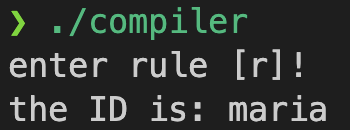
\includegraphics[width=0.25\textwidth]{fig/hello.png}
    \caption{hello maria输出}
\end{figure}

\subsection{文法文件编写}

在\texttt{grammar}目录下,创建\texttt{CactLexer.g4}和\texttt{CactParser.g4}两个文件,分别用于词法分析和语法分析。

\subsubsection{词法分析——CactLexer.g4}

首先声明这是个词法分析器:
\begin{lstlisting}[language=antlr]
    lexer grammar CactLexer;
\end{lstlisting}

随后按照讲义内容定义关键字,再按照优先级顺序定义运算符及其他符号:

\begin{lstlisting}[language=antlr]
    // Keywords
    Const: 'const' ;
    Int: 'int' ;
    Float: 'float' ;
    Char: 'char' ;
    Void: 'void' ;
    If : 'if';
    Else : 'else';
    While : 'while';
    Break : 'break';
    Continue : 'continue';
    Return : 'return';

    // Operators by precedence
    // Priority 1
    LeftBracket : '[' ;
    RightBracket : ']' ;
    LeftParenthesis : '(' ;
    RightParenthesis : ')' ;

    // Operators, ranked from highest to lowest priority
    // Priority 2
    ExclamationMark: '!';
    // Priority 3
    Asterisk: '*';
    Slash: '/';
    Percent: '%';
    // Priority 4
    // Binary Plus and Minus are also used as unary operators
    Minus: '-';
    Plus: '+';
    // Priority 5
    Less: '<' ;
    LessEqual: '<=' ;
    Greater: '>' ;
    GreaterEqual: '>=' ;
    // Priority 6
    LogicalEqual: '==' ;
    NotEqual: '!=' ;
    // Priority 7
    LogicalAnd: '&&' ;
    // Priority 8
    LogicalOr: '||' ;

    // Assignment, comma does not act as operator
    // The use of commas is limited to variable constant declarations, initial values, function declarations, and calls

    // Other tokens
    LeftBrace : '{' ;
    RightBrace : '}' ;
    Equal: '=' ;
    Comma: ',' ;
    Semicolon: ';' ;
\end{lstlisting}

接下来定义词法规则,包括标识符、常量、注释、空白字符,也都是讲义中的内容:

\begin{lstlisting}
    // Identifier and constants
    // CACT identifiers can consist of uppercase and lowercase letters, numbers, and underscores, but must begin with a letter or underscore
    Identifier: [a-zA-Z_][a-zA-Z0-9_]* ;
    // IntConst → DecimalConst | OctalConst | HexadecConst
    IntegerConstant: ('0' | [1-9][0-9]* | '0'[0-7]+ | '0'[xX][0-9a-fA-F]+);
    // CharConst  → "'"character"'"
    CharacterConstant: '\'' ( EscapeSequence | ~['\\] ) '\'';
    fragment EscapeSequence: '\\' ['"?\\abfnrtv0];
    // FloatConst
    FloatConstant: ([-]?       '.'[0-9]+                  |
                    [-]?[0-9]+ '.'[0-9]*                  |
                    [-]?       '.'[0-9]+  [eE][+-]?[0-9]+ |
                    [-]?[0-9]+('.'[0-9]*)?[eE][+-]?[0-9]+  )[fF];
    
    // Comments and white spaces
    LineComment: '//' ~[\r\n]* -> skip;
    BlockComment: '/*' .*? '*/' -> skip;
    NewLine: ('\r' ('\n')? | '\n') -> skip;
    WhiteSpaces : (' ' | '\t')+ -> skip;
\end{lstlisting}

下面对词法规则中的内容稍加解释:

\begin{enumerate}
    \item \textbf{标识符规则}
    
    \texttt{Identifier} 规则定义了 CACT 语言中标识符的格式:必须以字母或下划线开头,后面可以跟任意数量的字母、数字或下划线。
    
    \item \textbf{常量规则}
    
    代码定义了三种基本常量类型:
    \begin{enumerate}
        \item \texttt{IntegerConstant} 支持三种表示方式:
        \begin{itemize}
            \item 十进制:\texttt{0} 或以非零数字开头的数字序列
            \item 八进制:以 \texttt{0} 开头的八进制数字序列
            \item 十六进制:以 \texttt{0x} 或 \texttt{0X} 开头的十六进制数字序列
        \end{itemize}
        
        \item \texttt{CharacterConstant} 定义了字符常量,格式为单引号括起的单个字符,支持转义序列:
        \begin{itemize}
            \item 普通字符:任何非单引号和反斜杠的字符
            \item 转义字符:由 \texttt{EscapeSequence} 片段定义,包括常见转义序列如 \texttt{\textbackslash n}、\texttt{\textbackslash t} 等
        \end{itemize}
        
        \item \texttt{FloatConstant} 定义了浮点常量,必须以 \texttt{f} 或 \texttt{F} 结尾,支持多种格式:
        \begin{itemize}
            \item 可选负号加小数点加数字(如 \texttt{-.123f})
            \item 可选负号加数字加小数点加可选数字(如 \texttt{-42.f})
            \item 带指数的浮点数表示,使用 \texttt{e} 或 \texttt{E} 表示指数部分
        \end{itemize}
    \end{enumerate}
    
    \item \textbf{注释和空白字符}
    \begin{enumerate}
        \item 单行注释:以 \texttt{//} 开头,直到行尾的所有内容
        \item 块注释:以 \texttt{/*} 开头,以 \texttt{*/} 结尾的所有内容
        \item 换行符:支持 CR、LF 或 CRLF 格式
        \item 空白字符:包括空格和制表符
    \end{enumerate}
    
    所有这些注释和空白字符都使用 \texttt{-> skip} 指令,表示词法分析器在识别它们后会跳过。
\end{enumerate}

\subsubsection{语法分析——CactParser.g4}

同样先声明这是个语法分析器,然后使用\texttt{CactLexer}中定义的词法规则:

\begin{lstlisting}[language=antlr]
    parser grammar CactParser;

    options {
    tokenVocab=CactLexer;
    }
\end{lstlisting}

然后是声明和定义部分:

\begin{lstlisting}[language=antlr]
    // declaration & defination
    // 编译单元: CompUnit → [ CompUnit ] ( Decl | FuncDef )
    compilationUnit: (declaration | functionDefinition)*;
    // 声明: Decl → ConstDecl | VarDecl
    declaration: constantDeclaration | variableDeclaration;
    // 常量声明: ConstDecl → 'const' BType ConstDef { ',' ConstDef } ';'
    constantDeclaration: Const basicType constantDefinition (Comma constantDefinition)* Semicolon;
    // 基本类型: BType → 'int' | 'float' | 'char'
    basicType: Int | Float | Char;
    // 常量定义: ConstDef → Ident { '[' IntConst ']' } '=' ConstInitVal
    constantDefinition: Identifier (LeftBracket IntegerConstant RightBracket)* Equal constantInitializationValue;
    // 初始值: ConstInitVal → ConstExp | '{' [ ConstInitVal { ',' ConstInitVal } ] '}'
    constantInitializationValue: constantExpression | LeftBrace (constantInitializationValue (Comma constantInitializationValue)*)? RightBrace;
    // 变量声明: VarDecl → BType VarDef { ',' VarDef } ';'
    variableDeclaration: basicType variableDefinition (Comma variableDefinition)* Semicolon;
    // 变量定义: VarDef → Ident { '[' IntConst ']' } [ '=' ConstInitVal ]
    variableDefinition: Identifier (LeftBracket IntegerConstant RightBracket)* (Equal constantInitializationValue)?;
    // 函数定义FuncDef → FuncType Ident '(' [FuncFParams] ')' Block
    functionDefinition: functionType Identifier LeftParenthesis (functionFormalParameters)? RightParenthesis block;
    // 函数类型FuncType → 'void' | 'int' | 'float' | 'char'
    functionType: Void | Int | Float | Char;
    // 形参列表FuncFParams → FuncFParam { ',' FuncFParam }
    functionFormalParameters: functionFormalParameter (Comma functionFormalParameter)*;
    // 函数形参FuncFParam → BType Ident [ '[' IntConst? ']' { '[' IntConst ']' } ]
    functionFormalParameter: basicType Identifier (LeftBracket IntegerConstant? RightBracket (LeftBracket IntegerConstant RightBracket)*)?;
\end{lstlisting}

接着是语句和表达式部分:

\begin{lstlisting}[language=antlr]
    // statement & expression
    // 语句块: Block → '{' { BlockItem } '}'
    block: LeftBrace (blockItem)* RightBrace;
    // 语句块项: BlockItem → Decl | Stmt
    blockItem: declaration | statement;
    // 语句Stmt → LVal '=' Exp ';' | [ Exp ] ';' | Block | 'return' Exp? | 'if' '(' Cond ')' Stmt [ 'else' Stmt ] | 'while' '(' Cond ')' Stmt | 'break' ';' | 'continue' ';
    statement: leftValue Equal expression Semicolon
             | (expression)? Semicolon
             | block
             | Return expression? Semicolon
             | If LeftParenthesis condition RightParenthesis statement (Else statement)?
             | While LeftParenthesis condition RightParenthesis statement
             | Break Semicolon
             | Continue Semicolon;
    // 表达式: Exp → AddExp
    expression: addExpression;
    // 常量算式: ConstExp → AddExp
    constantExpression: addExpression;
    // 条件算式Cond → LOrExp
    condition: logicalOrExpression;
    // 左值算式LVal → Ident { '[' Exp ']' }
    leftValue: Identifier (LeftBracket expression RightBracket)*;
    // 数值Number → IntConst | CharConst | FloatConst
    number: IntegerConstant | CharacterConstant | FloatConstant;
    // 函数实参表FuncRParams → Exp { ',' Exp }
    functionRealParameters: expression (Comma expression)*;
    // PrimaryExp → '(' Exp ')' | LVal | Number
    primaryExpression: LeftParenthesis expression RightParenthesis
                      | leftValue
                      | number;
    // UnaryExp → PrimaryExp | ('+' | '-' | '!') UnaryExp | Ident '(' [ FuncRParams ] ')' 注:'!'仅出现在条件表达式中
    unaryExpression: primaryExpression
                    | (Plus | Minus | ExclamationMark) unaryExpression
                    | Identifier LeftParenthesis (functionRealParameters)? RightParenthesis;
    // MulExp → UnaryExp | MulExp (' *' | '/' | '%') UnaryExp
    multiplicativeExpression: unaryExpression | multiplicativeExpression (Asterisk | Slash | Percent) unaryExpression;
    // AddExp → MulExp | AddExp ('+'|'-') MulExp
    addExpression: multiplicativeExpression | addExpression (Plus | Minus) multiplicativeExpression;
    //  RelExp → AddExp | RelExp ('<' | '>' | '<=' | '>=') AddExp
    relationalExpression: addExpression | relationalExpression (Less | Greater | LessEqual | GreaterEqual) addExpression;
    //  EqExp → RelExp | EqExp ('==' | '!=') RelExp
    equalityExpression: relationalExpression | equalityExpression (LogicalEqual | NotEqual) relationalExpression;
    //  LAndExp → EqExp | LAndExp '&&' EqExp
    logicalAndExpression: equalityExpression | logicalAndExpression LogicalAnd equalityExpression;
    //  LOrExp → LAndExp | LOrExp '||' LAndExp
    logicalOrExpression: logicalAndExpression | logicalOrExpression LogicalOr logicalAndExpression;
\end{lstlisting}

这两个部分也都是讲义中的内容,不再加以详细解释。

\subsection{覆写ANTLR默认的文法错误处理机制}

我们需要更改项目根目录下\texttt{src}文件夹中的内容。首先是\texttt{main.cpp},添加头文件如下:

\begin{lstlisting}[language=C++]
    #include <iostream>     // 标准输入输出流
    #include <filesystem>   // 文件系统库(C++17)
    #include <fstream>      // 文件流
    
    #include "ANTLRInputStream.h"   // ANTLR 输入流
    #include "CactLexer.h"          // 词法分析器
    #include "CactParser.h"         // 语法分析器
    #include "include/syntax_error_listener.h"  // 自定义语法错误监听器
\end{lstlisting}

这当中,\texttt{ANTLRInputStream.h}、\texttt{CactLexer.h}和\texttt{CactParser.h}是我们在\texttt{grammar}目录下自动生成的文件,\texttt{syntax\_error\_listener.h}是我们自定义的语法错误监听器。

接着继续修改\texttt{main}函数中的内容。

先检查是否提供了正确的命令行参数。编译器需要一个输入文件作为参数,如果参数数量不为2(程序名称加一个文件路径),则显示使用说明并退出。

\begin{lstlisting}[language=C++]
    // 检查命令行参数
    if (argc != 2) {
        std::cerr << "Usage: " << argv[0] << " <input_file>" << std::endl << std::endl;
        return 1;
    }
\end{lstlisting}

然后尝试打开指定的源代码文件。如果文件无法打开,则输出错误信息并退出。同时,从完整路径中提取只包含文件名的部分,用于后续错误报告。

\begin{lstlisting}[language=C++]
    // 打开输入文件流
    std::ifstream stream(argv[1]);
    if (!stream) {
        std::cerr << "Error: Could not open file: " << argv[1] << std::endl << std::endl;
        return 1;
    }
    
    // 获取文件名(不包含路径)
    std::string filename = std::filesystem::path(argv[1]).filename().string();
\end{lstlisting}

接下来初始化ANTLR组件。

\begin{lstlisting}[language=C++]
    // 从文件流读取字符
    antlr4::ANTLRInputStream input(stream);

    // 词法分析器,将字符流转换为标记流
    CactLexer lexer(&input);

    // 标记缓冲区
    antlr4::CommonTokenStream tokens(&lexer);

    // 语法分析器,分析标记流构建语法树
    CactParser parser(&tokens);
\end{lstlisting}

移除默认的错误监听器,并添加自定义的错误监听器。

\begin{lstlisting}[language=C++]
    lexer.removeErrorListeners();
    parser.removeErrorListeners();

    cact_parser::CactErrorListener cact_error_listener;
    lexer.addErrorListener(&cact_error_listener);
    parser.addErrorListener(&cact_error_listener);
\end{lstlisting}

最后解析文件,进行三重检查,并捕获两种异常:

\begin{enumerate}
    \item 三重检查
    \begin{enumerate}
        \item 确保语法树成功创建
        \item 检查自定义错误监听器是否发现了语法错误
        \item 确保所有输入都已被消费(没有未匹配的输入)
    \end{enumerate}
    \item 两种异常
    \begin{enumerate}
        \item ANTLR特定的异常
        \item 其他标准异常
    \end{enumerate}
\end{enumerate}

\begin{lstlisting}[language=C++]
    try {
        // 解析输入文件
        antlr4::tree::ParseTree *tree = parser.compilationUnit();
        if (!tree) {
            std::cerr << "Error: Failed to parse input file." << std::endl;
            return 1;
        }
        // 检查是否有语法错误
        if (cact_error_listener.hasSyntaxError()) {
            std::cerr << filename << ": Syntax error detected." << std::endl << std::endl;
            std::cerr << "----------------------------------------" << std::endl<< std::endl; // 分隔线
            return 1;
        }

        // 检查是否还有未消费的 token
        if (tokens.LA(1) != antlr4::Token::EOF) {
            std::cerr << filename << ": Error: Unmatched input detected after parsing." << std::endl << std::endl;
            std::cerr << "----------------------------------------" << std::endl<< std::endl; // 分隔线
            return 1;
        }

        // 输出成功信息
        std::cout << filename << ": Parsing succeeded." << std::endl << std::endl;
        std::cerr << "----------------------------------------" << std::endl<< std::endl; // 分隔线
    }catch (const antlr4::RecognitionException &e) {
        // 处理 ANTLR 特定的异常
        std::cerr << "ANTLR Recognition error: " << e.what() << std::endl;
        std::cerr << filename << ": Parsing failed." << std::endl << std::endl;
        return 1;
    } 
    catch (const std::exception &e) {
        // 捕获异常并输出错误信息
        std::cerr << "Error while parsing file '" << argv[1] << "': " << e.what() << std::endl << std::endl;
        return 1;
    }
\end{lstlisting}

接下来讲讲检查语法错误的部分。我们在\texttt{syntax\_error\_listener.h}中定义了一个自定义的语法错误监听器类\texttt{CactErrorListener},它继承自ANTLR的\texttt{BaseErrorListener}类。这个类重写了\texttt{syntaxError}方法,以便在发生语法错误时输出详细的错误信息。

当语法出现错误时,\texttt{syntaxError}方法会被调用,我们在这个方法中输出错误信息。我们还设置了一个标志\texttt{has\_syntax\_error},用于指示是否发生了语法错误。

\begin{lstlisting}[language=C++]
    #ifndef CPLAB_SYNTAX_ERROR_LISTENER
    #define CPLAB_SYNTAX_ERROR_LISTENER
    
    #include "BaseErrorListener.h"
    
    namespace cact_parser
    {
        class CactErrorListener final : public antlr4::BaseErrorListener
        {
        public:
            // 语法错误监听器的构造函数
            void syntaxError(antlr4::Recognizer *recognizer, antlr4::Token *offendingSymbol,
                             size_t line, size_t charPositionInLine, const std::string &msg,
                             std::exception_ptr e) override;
    
            // 检查是否有语法错误
            bool hasSyntaxError();
    
        private:
            bool has_syntax_error = false; // 标志是否有语法错误
        };
    } // namespace cact_parser
    #endif // CPLAB_SYNTAX_ERROR_LISTENER
\end{lstlisting}

在\texttt{syntax\_error\_listener.cpp}中实现了这个类的成员函数,输出错误信息,包括错误消息、行号、字符位置和错误的符号。我们还提供了一个方法\texttt{hasSyntaxError},用于返回是否发生了语法错误。

\begin{lstlisting}[language=C++]
    namespace cact_parser {
        // 语法错误监听器的构造函数
        void CactErrorListener::syntaxError(antlr4::Recognizer *recognizer, antlr4::Token *offendingSymbol,
            size_t line, size_t charPositionInLine, const std::string &msg, std::exception_ptr e) {
            has_syntax_error = true; // 设置语法错误标志为true
            std::cerr << "Syntax Error Message: " << msg << std::endl; // 输出语法错误信息
            std::cerr << "Line: " << line << ", Position: " << charPositionInLine << std::endl; // 输出错误位置
            std::cerr << "Offending Symbol: " << (offendingSymbol ? offendingSymbol->getText() : "null") << std::endl; // 输出错误的符号
        }
        bool CactErrorListener::hasSyntaxError() {
            return has_syntax_error; // 返回语法错误标志
        }
    }
\end{lstlisting}

\subsection{测试结果}

编译得到编译器之后,对于给出的27个测试用例,我们编写了一个脚本来自动化测试。脚本会遍历\texttt{test}目录下的所有文件,并将每个文件的内容传递给编译器进行解析,并输出结果。

\begin{lstlisting}
    # 遍历 ./test 文件夹中的每个文件
    for file in ./test/samples_lex_and_syntax/*; do
      # 执行 ./build/compiler 命令,传递文件名作为第二个参数
      ./build/compiler "$file"
    done
\end{lstlisting}

测试结果如下:

\begin{figure}[H]
    \centering
    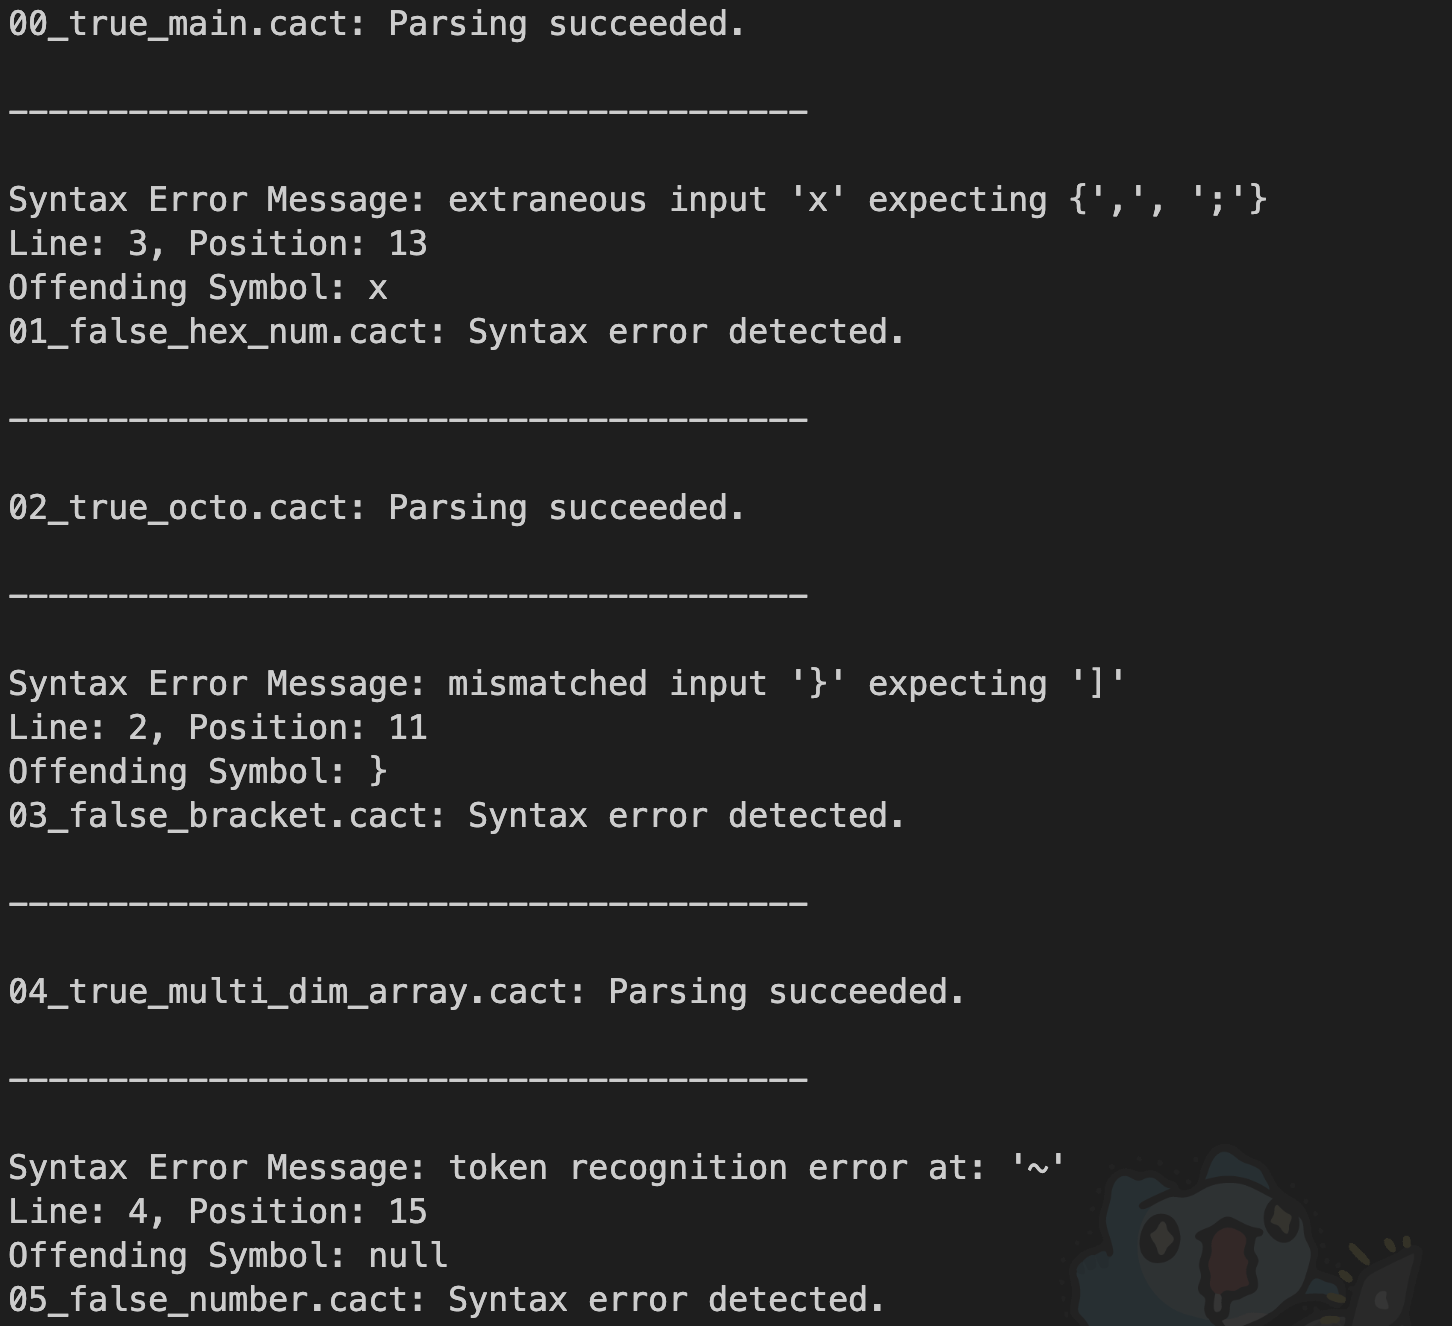
\includegraphics[width=0.7\textwidth]{fig/res00_05.png}
\end{figure}

\begin{figure}[H]
    \centering
    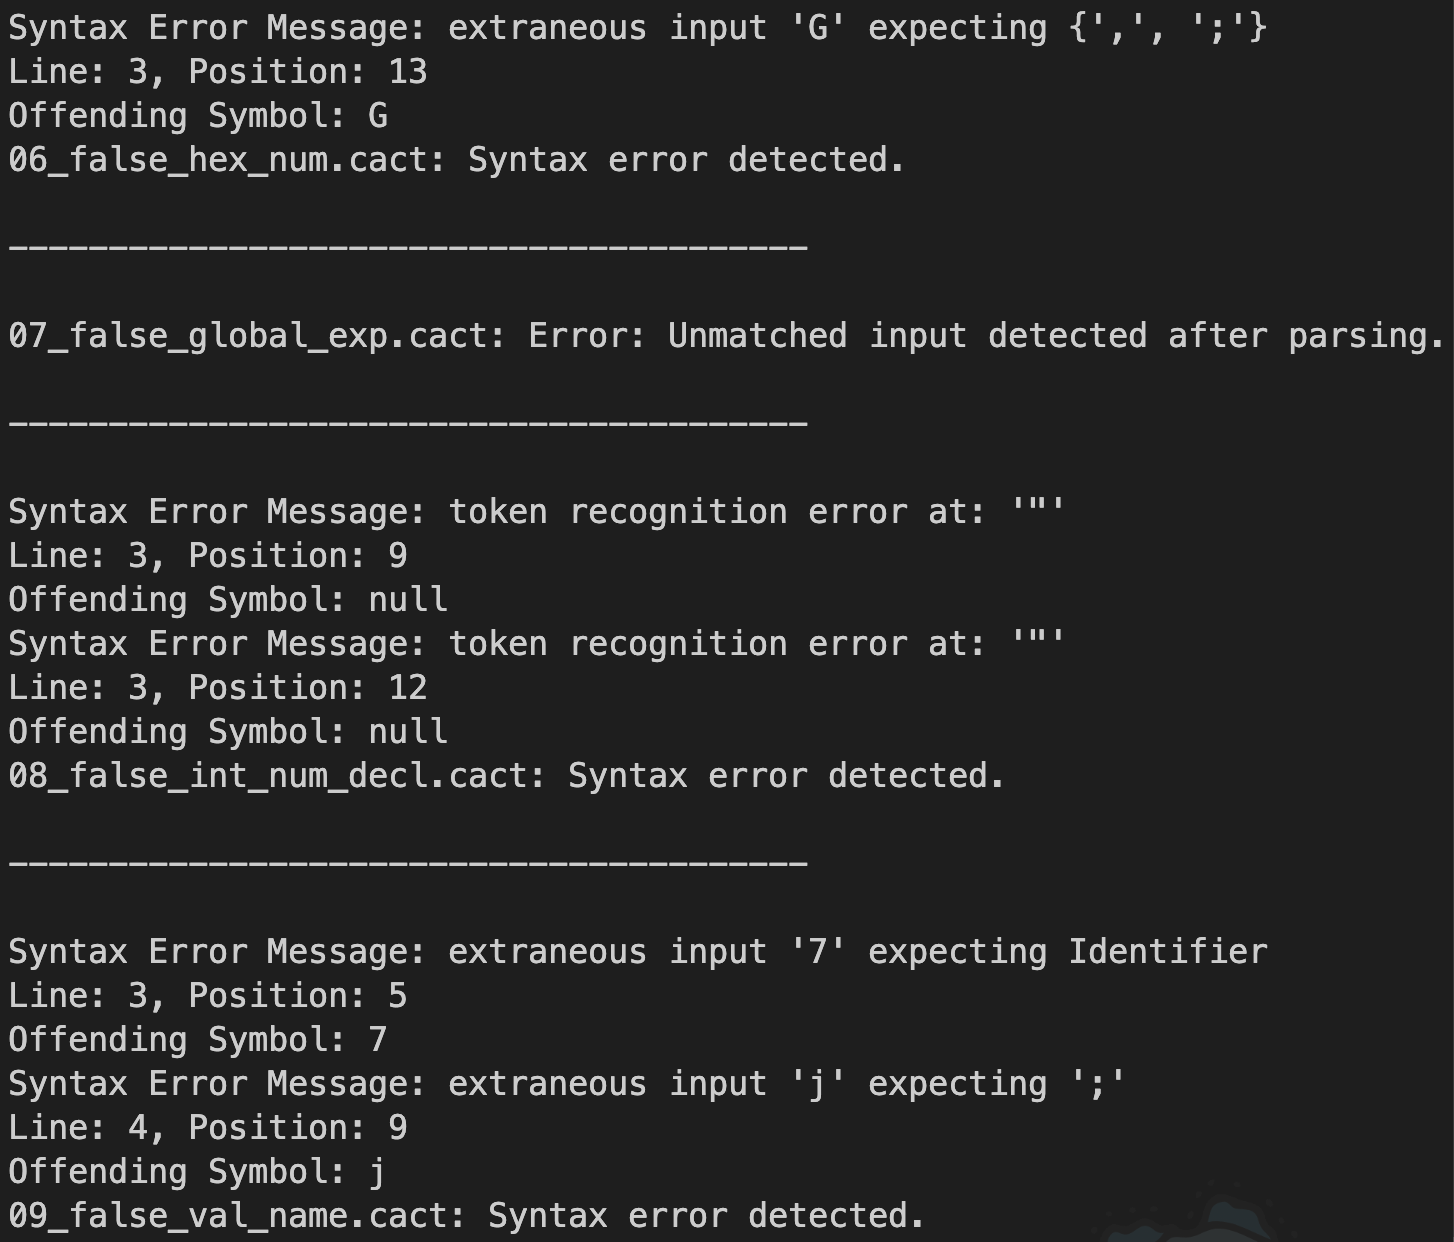
\includegraphics[width=0.7\textwidth]{fig/res06_09.png}
\end{figure}

\begin{figure}[H]
    \centering
    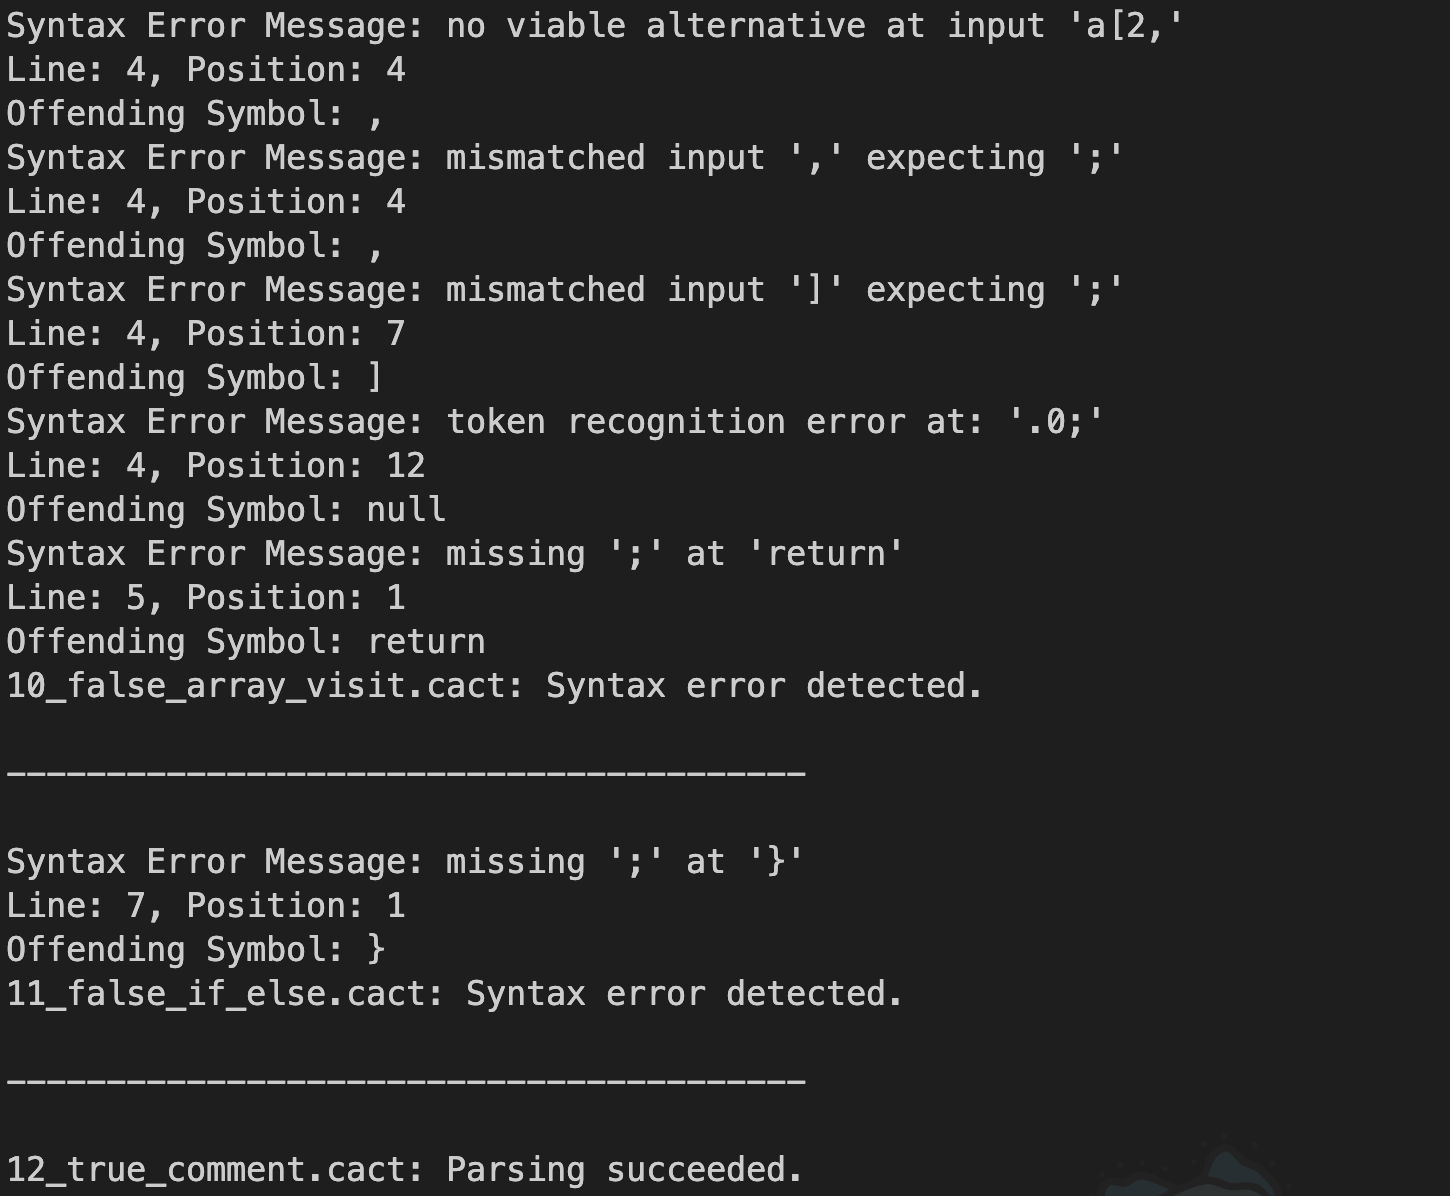
\includegraphics[width=0.7\textwidth]{fig/res10_12.png}
\end{figure}

\begin{figure}[H]
    \centering
    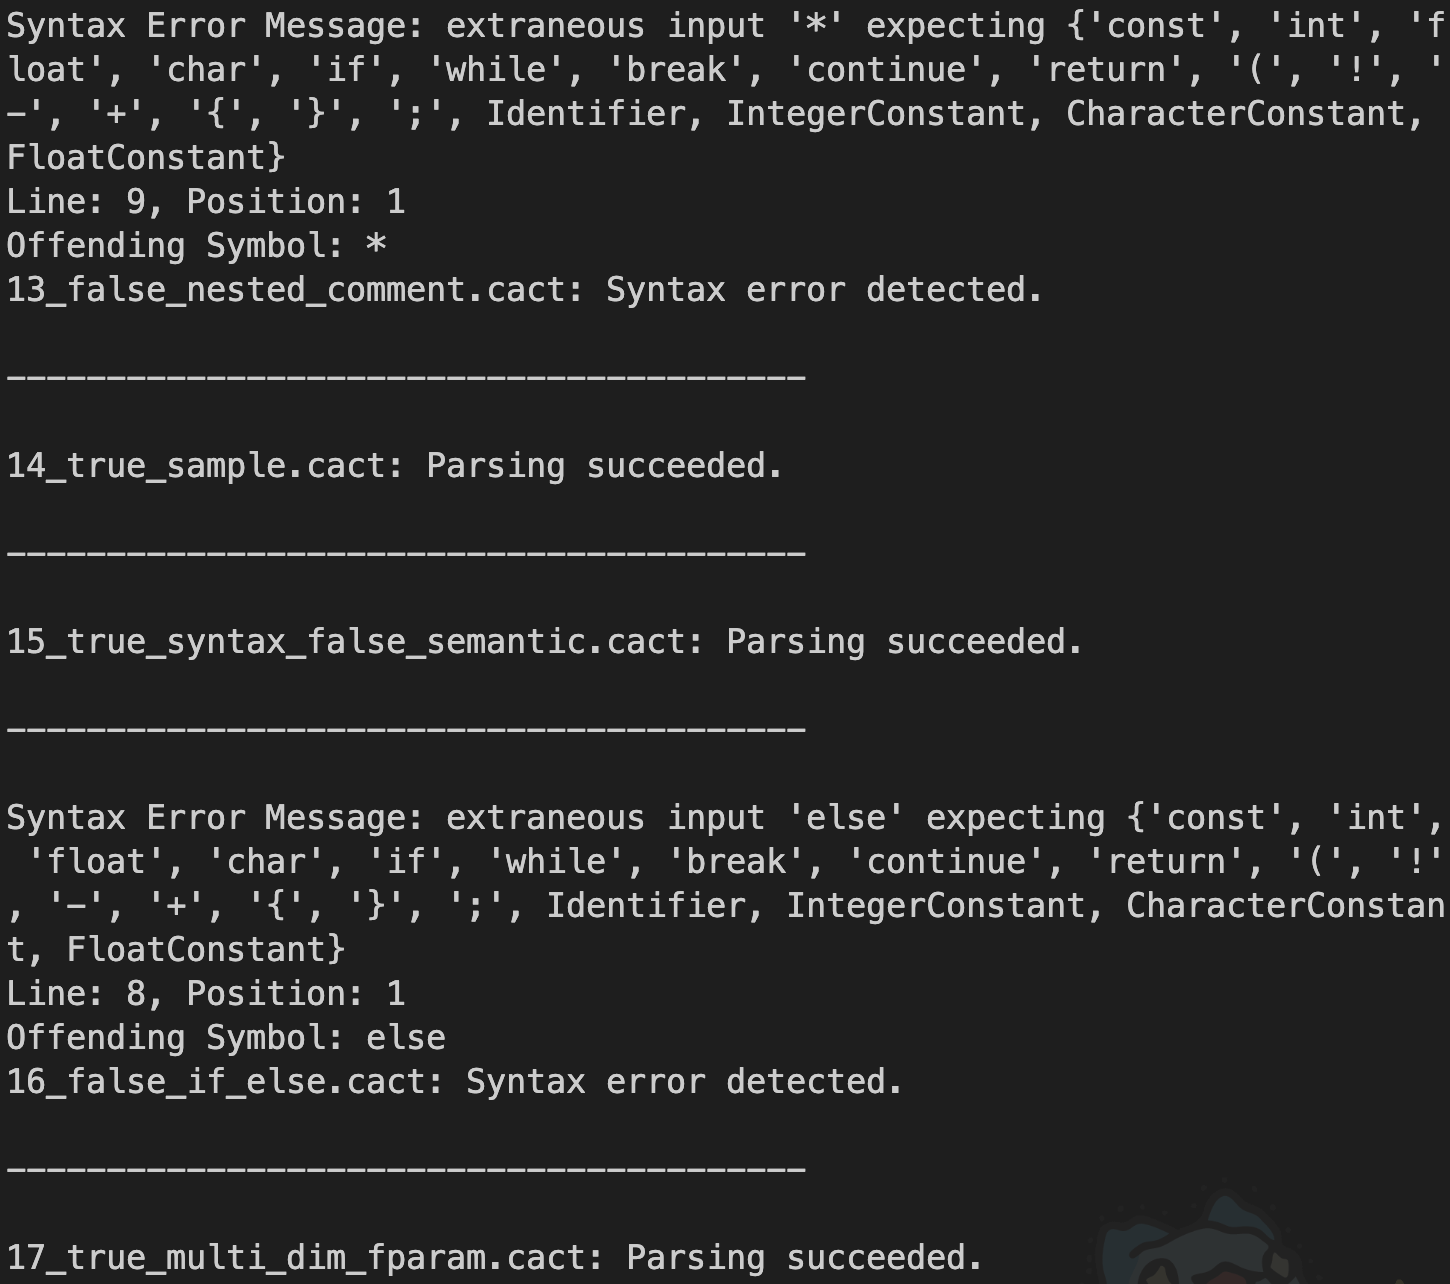
\includegraphics[width=0.7\textwidth]{fig/res13_17.png}
\end{figure}

\begin{figure}[H]
    \centering
    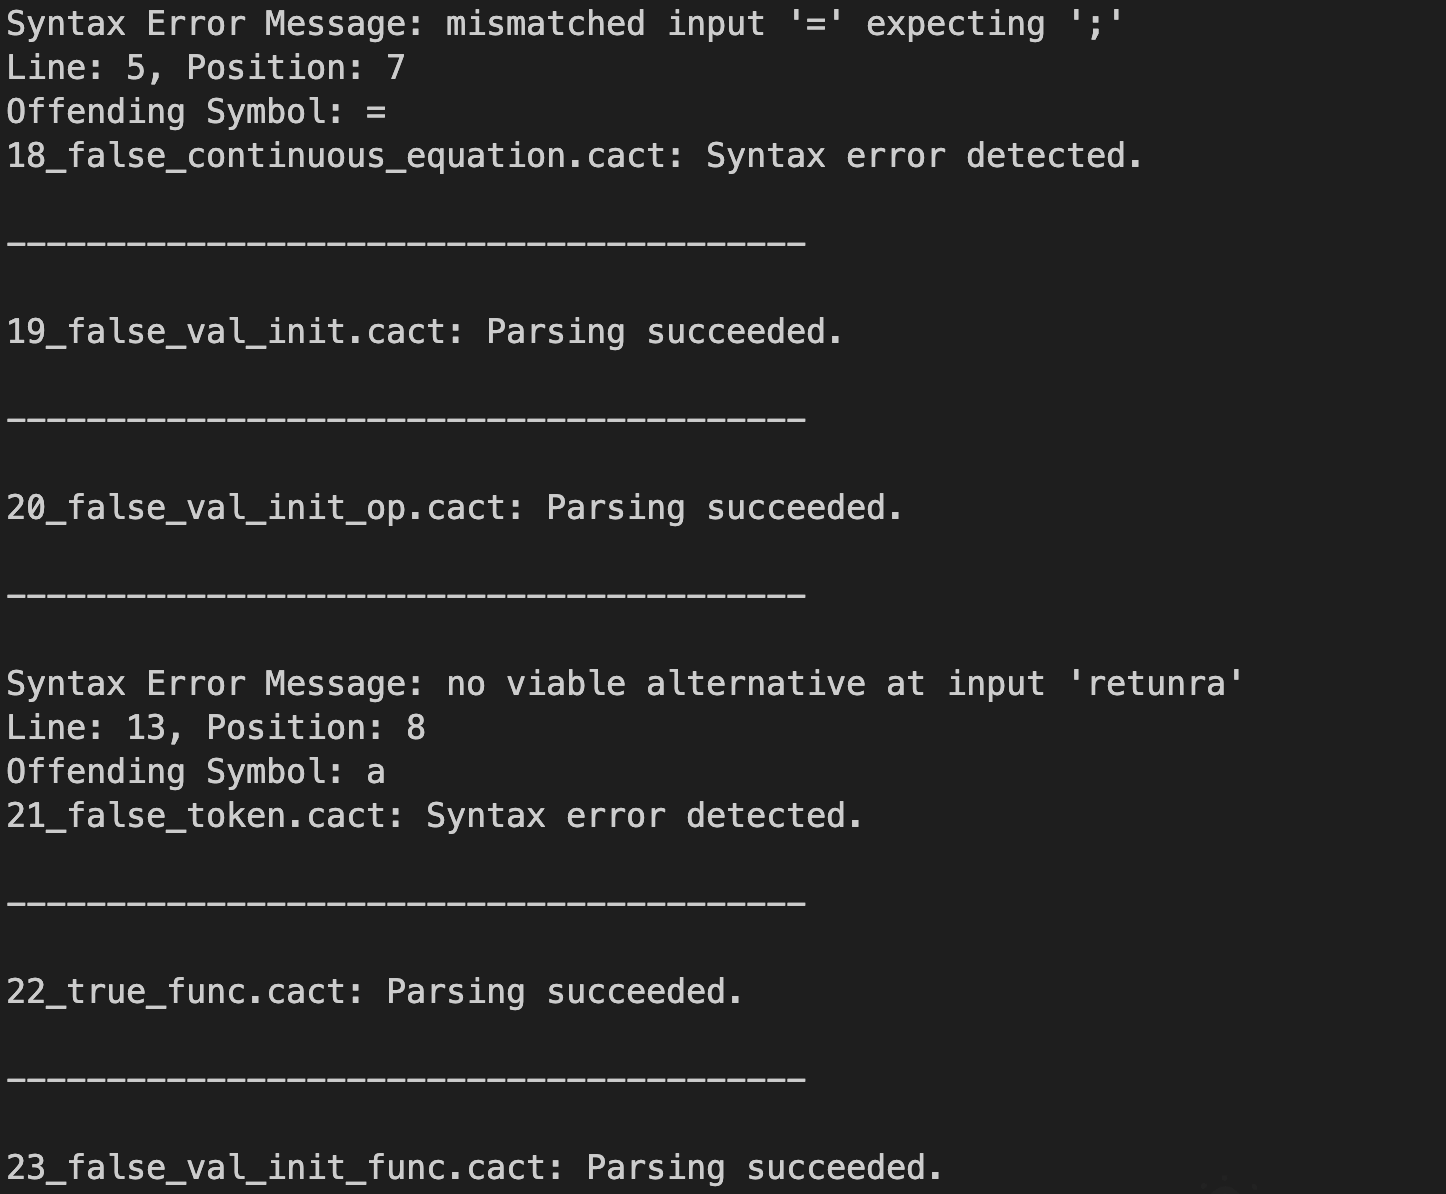
\includegraphics[width=0.7\textwidth]{fig/res18_23.png}
\end{figure}

\begin{figure}[H]
    \centering
    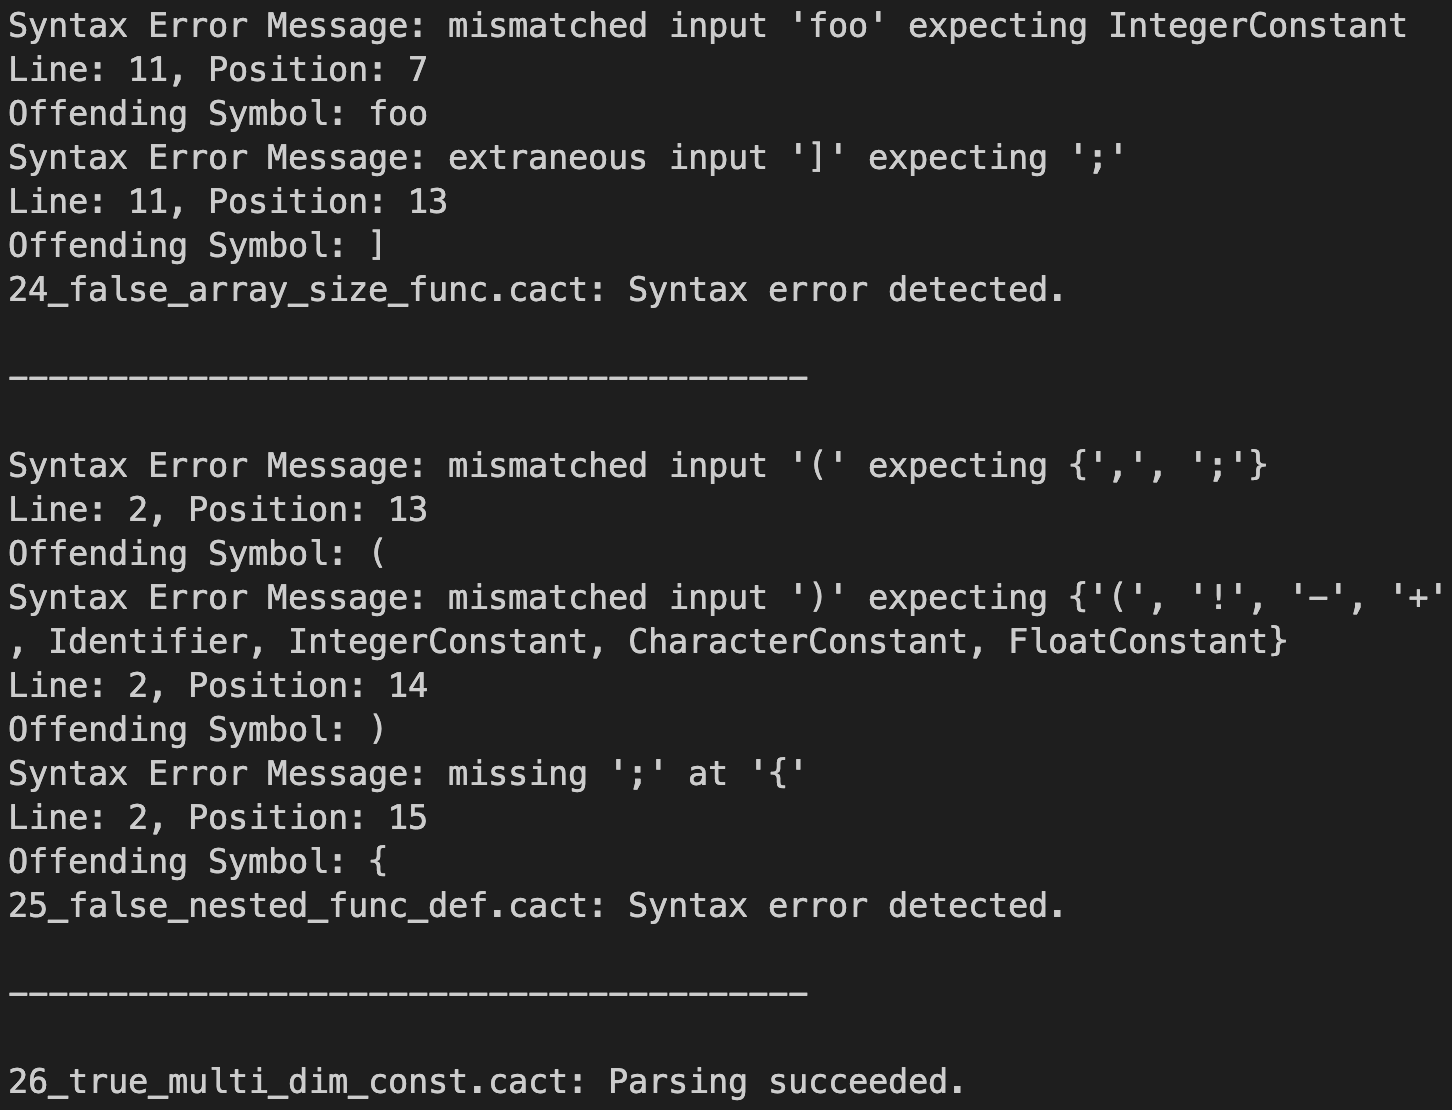
\includegraphics[width=0.7\textwidth]{fig/res24_26.png}
    \caption{测试结果}
\end{figure}

需要指出一点,样例19、20、23均应输出通过,这里样例的命名有误。如此可见,我们的编译器在词法和语法分析方面表现良好,能够正确处理各种样例。

\section{思考题}

\begin{enumerate}
    \item 如何设计编译器的目录结构?
    
    编译器的目录结构通常包括以下几个部分:
    \begin{enumerate}
        \item \texttt{src}:源代码目录,存放编译器的源代码文件。
        \item \texttt{grammar}:文法文件目录,存放ANTLR生成的文法文件。
        \item \texttt{test}:测试用例目录,存放测试用例和测试脚本。
        \item \texttt{deps}:依赖库目录,存放编译器所需的外部库和工具。
        \item \texttt{build}:构建目录,存放编译生成的可执行文件和中间文件。
    \end{enumerate}

    \item 如何把表达式优先级体现在文法设计中?
    
    在文法设计中,可以通过调整规则的定义顺序来体现表达式的优先级。举例如下:

    \begin{lstlisting}
        // 乘法优先级高于加法
        S -> E + F | E
        E -> E * F | F
        F -> id
    \end{lstlisting}

    在生成的解析树中,乘法操作会在加法操作之前进行解析,从而实现优先级。

    \item 如何设计数值常量的词法规则?
    
    数值常量分成整数常量、浮点常量、字符常量三种类型。在我们的代码中,这三种变量定义如下:

    \begin{lstlisting}
        IntegerConstant: ('0' | [1-9][0-9]* | '0'[0-7]+ | '0'[xX][0-9a-fA-F]+);

        CharacterConstant: '\'' ( EscapeSequence | ~['\\] ) '\'';
        fragment EscapeSequence: '\\' ['"?\\abfnrtv0];

        FloatConstant: ([-]?       '.'[0-9]+                  |
                        [-]?[0-9]+ '.'[0-9]*                  |
                        [-]?       '.'[0-9]+  [eE][+-]?[0-9]+ |
                        [-]?[0-9]+('.'[0-9]*)?[eE][+-]?[0-9]+  )[fF];
    \end{lstlisting}

    其中整数常量支持十进制、八进制和十六进制表示,字符常量用单引号括起来,浮点常量支持多种格式。
    

    \item 如何替换ANTLR的默认异常处理方法?
    
    我们可以通过覆写\texttt{BaseErrorListener}类中的\texttt{syntaxError}方法来实现自定义的异常处理。在这个方法中,我们可以输出更详细的错误信息,并设置一个标志来指示是否发生了语法错误。
\end{enumerate}

\section{实验总结}

本次实验主要是对编译器的词法分析和语法分析部分进行实现。通过使用ANTLR工具,我们能够快速地生成词法分析器和语法分析器,并且能够自定义错误处理机制。这是我们第一次接触编译器的实现,虽然过程有些繁琐,但通过实验,我们对编译器的工作原理有了更深入的理解。这使得我们在后续的实验中能够更好地进行语义分析和代码生成等工作。
\end{document}